\documentclass[dvipdfmx]{ujarticle}
\usepackage{eee}

\begin{document}
\title{平成29年 電磁気学II}
\date{}
\author{大山主朗}

\maketitle

\section*{平成29年 電磁気学II 第1回小テスト}

\section{以下の(a)及び(d)に示す物理定数は電磁気学を修めた者であれば常識的に覚えていなければならない数値である.それぞれの値を示せ.}
\begin{enumerate}[(a)]
	\item 真空の誘電率$\varepsilon_{0}:8.854 \times 10^{-12}\,\rm{F/m}$
	\item 真空の透磁率$\mu_{0}:1.257 \times 10^{-6}\,\rm{H/m}$
	\item 電子の電荷$e:-1.602 \times 10^{-19}\,\rm{C}$
	\item 電子の静止質量$m:9.109\times 10^{-31}\,\rm{kg}$
\end{enumerate}

\section{一辺の長さ$a$の正方形がある.点Aに$+q[\rm{C}]$,点Bに$+2q[\rm{C}]$,点Cに$−3q[\rm{C}]$,点Dに$−4q[\rm{C}]$,が点Oに$5q[\rm{C}]$の点電荷が存在するとき,点Oにある電荷にはたらく力$F$の大きさを求めよ.ただし,$q>0$とする.}
\begin{align*}
	\boldsymbol{F}_{A}&=\frac{1}{4\pi \varepsilon_{0}}\frac{5q^2}{\left(\left(\frac{a}{2}\right)^{2}+\left(-\frac{a}{2}\right)^{2}\right)^{3/2}} \left\{\frac{a}{2}\boldsymbol{i}-\frac{a}{2}\boldsymbol{j}\right\}\\
	\boldsymbol{F}_{B}&=\frac{1}{4\pi \varepsilon_{0}}\frac{10q^2}{\left(\left(\frac{a}{2}\right)^{2}+\left(\frac{a}{2}\right)^{2}\right)^{3/2}} \left\{\frac{a}{2}\boldsymbol{i}+\frac{a}{2}\boldsymbol{j}\right\}\\
	\boldsymbol{F}_{C}&=\frac{1}{4\pi \varepsilon_{0}}\frac{-15q^2}{\left(\left(-\frac{a}{2}\right)^{2}+\left(\frac{a}{2}\right)^{2}\right)^{3/2}} \left\{-\frac{a}{2}\boldsymbol{i}+\frac{a}{2}\boldsymbol{j}\right\}\\
	\boldsymbol{F}_{D}&=\frac{1}{4\pi \varepsilon_{0}}\frac{-20q^2}{\left(\left(-\frac{a}{2}\right)^{2}+\left(-\frac{a}{2}\right)^{2}\right)^{3/2}} \left\{-\frac{a}{2}\boldsymbol{i}-\frac{a}{2}\boldsymbol{j}\right\}\\
	\boldsymbol{F}&=\boldsymbol{F}_{A}+\boldsymbol{F}_{B}+\boldsymbol{F}_{C}+\boldsymbol{F}_{D}\\
	&=\frac{5q^{2}}{4\pi\varepsilon_{0}{ \left(\frac{a^{2}}{2^{2}}+\frac{a^{2}}{2^{2}}\right)^{3/2}}}\left\{\left(\frac{1}{2}a+a+\frac{3}{2}a+2a\right)\boldsymbol{i}+\left(-\frac{1}{2}a+a-\frac{3}{2}a+2a\right)\boldsymbol{j}\right\}\\
	&=\frac{5\sqrt{2}q^{2}}{2\pi\varepsilon_{0}a^{2}}\left(5\boldsymbol{i}+\boldsymbol{j}\right)\\
	|\boldsymbol{F}|&=\frac{\sqrt{2}q^{2}}{2\pi\varepsilon_{0}a^{2}}\sqrt{5^{2}+1}\\
	&=\frac{5\sqrt{52}}{2\pi\varepsilon_{0}a^{2}}q^{2}\,[\rm{N}]
\end{align*}

\section{一辺の長さ$a$の正方形がある.点Bに$+m[\rm{Wb}]$,点Cに$−3m[\rm{Wb}]$,点D に $+2m [\rm{Wb}]$,点Oに $−m[\rm{Wb}]$の点磁荷が存在するとき,点Aにできる磁界$H$の大きさを求めよ.ただし,$m >0$とする.}
\begin{align*}
	\boldsymbol{H}_{O}&=\frac{1}{4\pi \mu_{0}}\frac{-m}{\left(\left(-\frac{a}{2}\right)^{2}+\left(\frac{a}{2}\right)^{2}\right)^{3/2}} \left\{-\frac{a}{2}\boldsymbol{i}+\frac{a}{2}\boldsymbol{j}\right\}\\
	&=\frac{1}{4\pi \mu_{0}}\frac{-m}{\frac{a^{2}}{2\sqrt{2}}} \left\{-\frac{a}{2}\boldsymbol{i}+\frac{a}{2}\boldsymbol{j}\right\}\\
	&=\frac{-m\sqrt{2}}{4\pi \mu_{0}a^{2}}(-\boldsymbol{i}+\boldsymbol{j})\,[\rm{A/m}]\\
	\boldsymbol{H}_{B}&=\frac{1}{4\pi \mu_{0}}\frac{m}{\left(a^{2} \right)^{3/2}}a\boldsymbol{j}\\
	&=\frac{m}{4\pi \mu_{0}a^{2}}\boldsymbol{j}\,[\rm{A/m}]\\
	\boldsymbol{H}_{C}&=\frac{1}{4\pi \mu_{0}}\frac{-3m}{\left((-a)^{2}+a^{2} \right)^{3/2}}\left\{ -a \boldsymbol{i}+a\boldsymbol{j}\right\}\\
	&=\frac{-3m}{8\sqrt{2} \pi \mu_{0} a^{2}}\left( -\boldsymbol{i}+\boldsymbol{j}\right)\,[\rm{A/m}]\\
	\boldsymbol{H}_{D}&=\frac{1}{4\pi \mu_{0}}\frac{2m}{\left((-a)^{2} \right)^{3/2}}\left(-a\boldsymbol{i}\right)\\
	&=-\frac{m}{2\pi \mu_{0}a^{2}}\boldsymbol{i}\,[\rm{A/m}]\\
	\boldsymbol{H}_{A}&=\boldsymbol{H}_{O}+\boldsymbol{H}_{B}+\boldsymbol{H}_{C}+\boldsymbol{H}_{D}\\
	&=\frac{m}{2\pi \mu_{0}a^{2}}\left\{\left(\frac{\sqrt{2}}{2}+\frac{3}{4\sqrt{2}}-1\right)\boldsymbol{i}+\left(-\frac{\sqrt{2}}{2}+\frac{1}{2}-\frac{3}{4\sqrt{2}}\right)\boldsymbol{j} \right\}\\
	&=\frac{m}{16\pi \mu_{0}a^{2}}\left\{\left(7\sqrt{2}-8\right)\boldsymbol{i}+\left(4-7\sqrt{2}\right)\boldsymbol{j} \right\}\\
	&=\frac{m}{16\pi \mu_{0}a^{2}}\sqrt{(7\sqrt{2}-8)^{2}+(4-7\sqrt{2})^{2}}\\
	&=\frac{m}{16\pi \mu_{0}a^{2}}\sqrt{(7\sqrt{2}-8)^{2}+(4-7\sqrt{2})^{2}}
\end{align*}

\section{真空中に単磁荷$m$が存在する.ただし$m<0$とする.このとき以下の問いに答えよ.}
\begin{enumerate}[(a)]
	\item 点磁荷$m$が,距離$r$の位置に作る磁界$H$を求めよ.
	\begin{align*}
		H&=\frac{m}{4 \pi \mu_{0} r^{2}}\,[\rm{A/m}]
	\end{align*}
	\item 点磁荷$m$が作る磁界の様子を磁力線を用いて図示せよ.
	\begin{figure}[h]
	\centering
	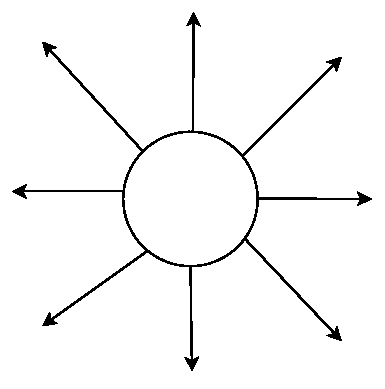
\includegraphics[scale=1]{/Users/ohyamasan/Downloads/efig.pdf}
	\end{figure}
	\item 点磁荷$m$から距離$r$の位置における磁束密度$B$を求めよ.
	\begin{align*}
		B&=\mu_{0} H=\frac{m}{4 \pi r^{2}}\,[\rm{T}]
	\end{align*}
	\item 点磁荷$m$から距離$r$の位置を通過する磁束$\Phi$を磁束密度$B$より求めよ.
	\begin{align*}
		\Phi&=BS=m\,[\rm{Wb/m}]
	\end{align*}
\end{enumerate}

\section{$xy$直交座標系において,同量異符号の点磁荷$\pm m$が距離$l$に固定された磁気双極子が存在する.このとき以下の問いに答えよ.ただし,$x$ 方向の基準ベクトルを$\boldsymbol{i}$,$y$方向の基準ベクトルを$\boldsymbol{j}$とする}
\begin{enumerate}[(a)]
	\item 点Aに存在する磁荷$-m$が点P$(x_0,y_0)$に作る磁界$\boldsymbol{H}_{1}$を求めよ.
	\begin{align*}
		\boldsymbol{H}_{1}&=\frac{1}{4\pi \mu_{0}}\frac{-m}{\left(\left(x_{0}+\frac{l}{2}\right)^{2}+y_{0}^{2}\right)^{3/2}} \left\{ \left(x_{0}+\frac{l}{2}\right)\boldsymbol{i}+y_{0}\boldsymbol{j}\right\}\,[\rm{A/m}]
	\end{align*}
	\item 点Bに存在する磁荷$+m$が点P$(x_0,y_0)$に作る磁界$\boldsymbol{H}_{2}$を求めよ.
	\begin{align*}
		\boldsymbol{H}_{2}&=\frac{1}{4\pi \mu_{0}}\frac{m}{\left(\left(x_{0}-\frac{l}{2}\right)^{2}+y_{0}^{2}\right)^{3/2}} \left\{ \left(x_{0}-\frac{l}{2}\right)\boldsymbol{i}+y_{0}\boldsymbol{j}\right\}\,[\rm{A/m}]
	\end{align*}
	\item 点Pでの磁界$\boldsymbol{H}$を求めよ.
	\begin{align*}
		\boldsymbol{H}&=\boldsymbol{H}_{1}+\boldsymbol{H}_{2}\\
		&=\frac{m}{4\pi \mu_{0}}\left[\frac{-1}{\left(\left(x_{0}+\frac{l}{2}\right)^{2}+y_{0}^{2}\right)^{3/2}} \left\{ \left(x_{0}+\frac{l}{2}\right)\boldsymbol{i}+y_{0}\boldsymbol{j}\right\}+\frac{1}{\left(\left(x_{0}-\frac{l}{2}\right)^{2}+y_{0}^{2}\right)^{3/2}} \left\{ \left(x_{0}-\frac{l}{2}\right)\boldsymbol{i}+y_{0}\boldsymbol{j}\right\}\right]\,[\rm{A/m}]
	\end{align*}
	\item 磁気双極子モーメント$\boldsymbol{M}$を求めよ.
	\begin{align*}
		\boldsymbol{M}&=m\boldsymbol{l}\\
		&=ml\boldsymbol{i}\,[\rm{Wb\cdot m}]
	\end{align*}
	\item 点Pが原点Oより十分遠方にあると仮定すると,$\sqrt{(x_{0}-l/2)^{2}+y_{0}^{2}}\simeq \sqrt{x_{0}^{2}+y_{0}^{2}}$及び$\sqrt{(x_{0}+l/2)^{2}+y_{0}^{2}} \simeq \sqrt{x_{0}^{2}+y_{0}^{2}}$と近似できる.このことを用いて(c)にて得た磁界$\boldsymbol{H}$を簡略化せよ.
	\begin{align*}
		\boldsymbol{H}&\simeq -\frac{1}{4\pi \mu_{0}}\frac{ml}{\left(x_{0}^{2}+y_{0}^{2}\right)^{3/2}} \boldsymbol{i}\,[\rm{A/m}]\\
		&\left(=-\frac{\boldsymbol{M}}{4\pi \mu_{0}r^{3}}\,[\rm{A/m}]\right)
	\end{align*}
	\item $y$方向に一様な磁界$\boldsymbol{H}_{0}$が存在するとき,磁気双極子にはたらくトルク$T$を求めよ.
	\begin{align*}
		\boldsymbol{T}&=\boldsymbol{M}H_{0}\sin \theta \\
		&=ml\boldsymbol{i}\sin \frac{\pi}{2}\\
		&=ml\boldsymbol{i}\\
		|\boldsymbol{T}|&=ml\,[\rm{Wb\cdot m}]
	\end{align*}
\end{enumerate}

\section{磁化されていない強磁性体に磁界$H$を外部から印加し,強磁性体内部での磁束密度$B$を観測すると,図3に示すような結果が得られた.このとき,図中の行程1:点$\rm{O}\to$点$\rm{P_{1}}$,行程 2:点$\rm{P_{1}}\to$点$\rm{P_{2}}$,行程3:点$\rm{P_{2}}\to$点$\rm{P_{3}}$,行程4:点$\rm{P_{3}}\to$点P4,行程5:点P4 $\to$点$\rm{P_{5}}$, 行程6:点$\rm{P_{5}}\to$点P6,行程7:点$\rm{P_{6}}\to$点P1の7つの行程に着目して,測定結果を説明せよ.}

\section{強磁性体,常磁性体,反磁性体の3つの磁性体の性質を,比透磁率と磁化率を用いて説明せよ.}
強磁性体は磁化率が0よりかなり大きく,透磁率が1よりかなり大きい磁性体を指す.そのため,磁界と同じ方向に磁化され,その大きさも大きい.

常磁性体は磁化率が0より大きく,透磁率は1未満の磁性体を指す.そのため,磁界と同じ方向に磁化され,その大きさは大きくない.

反磁性体は磁化率が0よりかなり小さく,透磁率が1よりかなり小さい磁性体を指す.そのため,磁界と逆方向に磁化され,その大きさは小さい.

\clearpage
\setcounter{section}{0}
\section*{平成29年 電磁気学II 第2回小テスト}
\section{以下の(a)及び(d)に示す物理定数は電磁気学を修めた者であれば常識的に覚えていなければならない数値である.それぞれの値を示せ.}
\begin{enumerate}[(a)]
	\item 真空の誘電率$\varepsilon_{0}:8.854 \times 10^{-12}\,\rm{F/m}$
	\item 真空の透磁率$\mu_{0}:1.257 \times 10^{-6}\,\rm{H/m}$
	\item 電子の電荷$e:-1.602 \times 10^{-19}\,\rm{C}$
	\item 電子の静止質量$m:9.109\times 10^{-31}\,\rm{kg}$
\end{enumerate}

\section{$xyz$直角座標空間において,原点Oを含む$xy$平面に半径$a$の円形ループ電流$I$が流れている.このとき,原点Oに発生する磁界$\boldsymbol{H}$を求めよ.}
\begin{align*}
	\boldsymbol{H}&=\oint d\boldsymbol{H}\\
	円周上に&線素ベクトルd\boldsymbol{l}をとる.\\
	ここで,円周上のどの点&でもd\boldsymbol{H}の向きが同じなので,\\
	H&=\oint dH\\
	&=\oint \frac{I\sin \theta }{4\pi r^{2}}dl\\
	&=\frac{I\sin \frac{\pi}{2} }{4\pi r^{2}}\cdot 2\pi r\\
	&=\frac{I}{2r}\\
	&=\frac{I}{2a}\,[\rm{A/m}]\quad 上向き\\
	\boldsymbol{H}&=\frac{I}{2a}\boldsymbol{k}\,[\rm{A/m}]
\end{align*}

\section{$xyz$直角座標空間において,原点Oを含む$xy$平面に半径$a$の円形ループ電流$I$が流れている.このとき,$z$軸上の点$\rm{P}(0, 0, h)$に発生する磁界$\boldsymbol{H}$を求めよ.}
\begin{align*}
	y>0に円周上の&微小磁界d\boldsymbol{H}_{1}を\\
	y<0に円周上の&微小磁界d\boldsymbol{H}_{2}を考える.\\
	またそれぞれの&線素ベクトルをd\boldsymbol{l}ととる.\\
	ここで,d\boldsymbol{H}_{1}とd\boldsymbol{H}_{2}の外積より,&2つの磁界は打ち消される方向となっているため,\\
	d\boldsymbol{H}_{1}とd\boldsymbol{H}_{2}を合成した&磁界をd\boldsymbol{H}とする.(\phi:d\boldsymbol{H}_{2}とd\boldsymbol{H}のなす角)\\
	|d\boldsymbol{H}_{1}|=|d\boldsymbol{H}_{2}|&=\frac{Idl}{4\pi r^{2}}\sin \theta\\
	&=\frac{Idl}{4\pi (a^{2}+h^{2})}\\
	d\boldsymbol{H}&=2d\boldsymbol{H}_{1}\cos \phi\\
	&=2d\boldsymbol{H}_{1}\frac{a}{r}\\
	&=2d\boldsymbol{H}_{1}\frac{a}{\sqrt{a^{2}+h^{2}}}\\
	|d\boldsymbol{H}|&=2|d\boldsymbol{H}_{1}|\frac{a}{\sqrt{a^{2}+h^{2}}}\\
	&=\frac{aIdl}{2\pi (a^{2}+h^{2})^{3/2}}\\
	\boldsymbol{H}&=\oint d\boldsymbol{H}_{1}\\
	|\boldsymbol{H}|&=\frac{1}{2}\oint|d\boldsymbol{H}|\\
	&=\frac{1}{2}\oint \frac{aIdl}{2\pi (a^{2}+h^{2})^{3/2}}\\
	&=\frac{1}{2}\cdot \frac{aI}{2\pi (a^{2}+h^{2})^{3/2}} \cdot 2\pi a\\
	&=\frac{a^{2}I}{2 (a^{2}+h^{2})^{3/2}}\,[\rm{A/m}]\quad 上向き\\
	\boldsymbol{H}&=\frac{a^{2}I}{2(a^{2}+h^{2})^{3/2}}\boldsymbol{k}\,[\rm{A/m}]
\end{align*}

\section{$xyz$直角座標空間において,$y$軸上の点$\rm{A}(0, c_{1}, 0)$から点$\rm{B}(0, c_{2}, 0)$まで$y$軸に沿って直線状に流れる電流$I$がある.このとき,$x$軸上の点$\rm{P}(a, 0, 0)$に発生する磁界$\boldsymbol{H}$を求めよ.また,電流$I$の始点 Aと終点Bの座標がそれぞれ$(0, -\infty, 0), (0, \infty, 0)$となった場合の点$\rm{P}$に発生する磁界$\boldsymbol{H}$を求めよ.}
\begin{align*}
	x方向,y方向,z方向の&基底ベクトルをそれぞれ\boldsymbol{i},\boldsymbol{j},\boldsymbol{k}とする\\
	この時&d\boldsymbol{l}=dy\boldsymbol{i}, \boldsymbol{r}=a\boldsymbol{i}-y\boldsymbol{j}\\
	d\boldsymbol{l}\times \boldsymbol{r}&=
	\begin{vmatrix}
	\boldsymbol{i} & \boldsymbol{j} & \boldsymbol{k}\\
	0 &dy & 0\\
	a & -y &0
	\end{vmatrix}
	=
	\begin{vmatrix}
	\boldsymbol{i}  & \boldsymbol{k}\\
	a & 0
	\end{vmatrix}
	=-ady\boldsymbol{k}\\
	\boldsymbol{H}&=\int_{C} d\boldsymbol{H}\\
	&=-\int_{C} \frac{aI\boldsymbol{k}}{4\pi(a^{2}+y^{2})^{3/2}}dy\\
	&=-\int_{c_{1}}^{c_{2}} \frac{aI\boldsymbol{k}}{4\pi(a^{2}+y^{2})^{3/2}}dy\\
	h&=a\tan \theta と置換する.\\
	\frac{dh}{d\theta}&=\frac{a}{\cos ^{2}\theta } \quad \therefore dh=\frac{a}{\cos ^{2}\theta }d\theta \\
	また積分範囲は&c_{1}\to c_{2}から\alpha-\frac{\pi}{2} \to \beta -\frac{\pi}{2}に変更される.\\
	&=-\int_{\alpha-\frac{\pi}{2}}^{\beta -\frac{\pi}{2}} \frac{a^{2}I}{4\pi a^{3}(1+\tan^{2}\theta)^{3/2}}\boldsymbol{j} \frac{a}{\cos ^{2}\theta }d\theta\\
	&=-\frac{I}{4\pi} \boldsymbol{j} \int_{\alpha-\frac{\pi}{2}}^{\beta -\frac{\pi}{2}} \frac{1}{(1+\tan^{2}\theta)^{3/2}} \frac{1}{\cos ^{2}\theta }d\theta\\
	&=-\frac{I}{4\pi a} \boldsymbol{j} \int_{\alpha-\frac{\pi}{2}}^{\beta -\frac{\pi}{2}} \frac{1}{(\frac{1}{\cos^{2} \theta })^{3/2}} \frac{1}{\cos ^{2}\theta }d\theta\\
	&=-\frac{I}{4\pi a} \boldsymbol{j} \int_{\alpha-\frac{\pi}{2}}^{\beta -\frac{\pi}{2}} \cos \theta d \theta \\\
	&=-\frac{I}{4\pi a} \boldsymbol{j} \left[\sin \theta  \right]_{\alpha-\frac{\pi}{2}}^{\beta -\frac{\pi}{2}}\\
	&=-\frac{I}{4\pi a} \boldsymbol{j} \left\{\sin \left(\beta -\frac{\pi}{2}\right) -\sin \left(\alpha-\frac{\pi}{2}\right) \right\}\\
	&=-\frac{I}{4\pi a} \boldsymbol{j}\left(-\cos \beta +\cos \alpha \right)\\
	&=-\frac{I}{4\pi a} \boldsymbol{j}\left(\cos \alpha -\cos \beta \right)\,[\rm{A/m}]\\
	始点Aと終点B&の座標がそれぞれ(0, -\infty, 0), (0, \infty, 0)の場合は\\
	\alpha=0,&\beta =\pi であるので\\
	\boldsymbol{H}&=-\frac{I}{4\pi a}\cdot 2 \boldsymbol{j}\\
	&=-\frac{I}{2\pi a} \boldsymbol{j}\,[\rm{A/m}]
	\end{align*}


\section{$xyz$直角座標空間において,原点Oに発生する磁界$\boldsymbol{H}$を求めよ.ただし,$a$を正の実定数とし,電流$I$が流れる経路は3つの経路$C_{1}\sim C_{3}$を通っており,それぞれの経路は以下のように定義されるものとする.}
\begin{itemize}
	\item $C_{1}:$$y$軸に沿って$(0, -\infty, 0)$から$(0, -a, 0)$へ進む経路
	\item $C_{2}$:$x=\sqrt{a^{2}-y^{2}}, z=0$に沿って$(0, -a, 0)$から$(a, 0, 0)$を通り$(0, a, 0)$へ進む経路.
	\item $C_{3}$:$y$軸に沿って$(0, a, 0)$から$(0, \infty, 0)$へ進む経路
\end{itemize}
\begin{align*}
	x方向,y方向,z方向の基底ベクトル&をそれぞれ\boldsymbol{i},\boldsymbol{j},\boldsymbol{k}とする\\
	|\boldsymbol{H}}|&=\oint |d\boldsymbol{H}_{a}|\\
	&=\frac{I}{4\pi r^{2}}\sin \frac{\pi}{2} \oint dl\\
	&=\frac{I}{4\pi r^{2}}\pi r\\
	&=\frac{I}{4r}\,[\rm{A/m}]\\
	d\boldsymbol{l}\times \boldsymbol{r}&より \\
	\boldsymbol{H}&=-\frac{I}{4a}\boldsymbol{k}\,[\rm{A/m}]\\
	また\theta=0となる&半直線部分は,\sin \theta =0となり,磁束は0\,[\rm{A/m}]\\
	\end{align*}


\section{$xyz$直角座標空間において,原点Oに発生する磁界$\boldsymbol{H}$を求めよ.ただし,$a$を正の実定数とし,電流$I$が流れる経路は5つの経路$C_{1}\sim C_{5}$を通っており,それぞれの経路は以下のように定義されるものとする.}
\begin{itemize}
	\item $C_{1}$:$y=-x,z=-a(x<0, y>0)$に沿って$(-\infty, \infty, -a)$から$(0, 0, -a)$へ進む経路
	\item $C_{2}$:$x^{2}+z^{2}=a^{2},y=0(x>0, z<0)$に沿って$(0, 0, -a)$から$(a, 0, 0)$へ進む経路
	\item $C_{3}$:$x^{2}+y^{2}=a^{2},z=0(x>0, y>0)$に沿って$(a, 0, 0)$から$(0, a, 0)$へ進む距離
	\item $C_{4}$:$y^{2}+z^{2}=a^{2},x=0(y>0, z>0)$に沿って$(0, a, 0)$から$(0, 0, a)$へ進む距離
	\item $C_{5}$:$y=-x, z=a(x>0. y<0)$に沿って$(0, 0, a)$から$(\infty, -\infty, a)$へ進む経路
\end{itemize}
\begin{align*}
\end{align*}

\section{無限長直線電流$I$が流れているとき,電流$I$から距離$a$の位置に発生する磁界$H$をアン
ペールの法則を用いて求めよ.}
\begin{align*}
\end{align*}

\clearpage
\setcounter{section}{0}
\section*{平成29年 電磁気学II 前期期末試験}
\end{document} 